\chapter{Módulo 3 – Trilha de Segurança de Dispositivos Móveis e Automação (75 Horas)}
\label{chap:modulo3}

A \textbf{Trilha de Segurança de Dispositivos Móveis e Automação de Validações} aborda a defesa em profundidade da plataforma Android. Os residentes aprendem a modelar vetores de ataque, auditar superfícies expostas, desvendar os mecanismos de proteção do kernel Linux (SELinux e Sandbox), explorar o isolamento criptográfico por hardware (\textit{StrongBox} e \textit{Keystore}) e automatizar verificações contínuas em pipelines DevSecOps.

---

\section{Introdução à Cibersegurança, Modelagem de Ameaças e Vulnerabilidades (35h)}

\begin{pedagogico}{Objetivo Pedagógico da Disciplina}
Capacitar os residentes para mapear superfícies de ataque em ecossistemas móveis, aplicar a metodologia STRIDE para modelagem formal de ameaças, identificar falhas de implementação no código-fonte e aplicar técnicas de hardening de aplicação e ofuscação.
\end{pedagogico}

\subsection{Metodologia de Modelagem de Ameaças: STRIDE}
O framework STRIDE, desenvolvido originalmente pela Microsoft e amplamente adotado na indústria de software crítico, categoriza ameaças em seis classes fundamentais:
\begin{table}[htbp]
\centering
\small
\begin{tabularx}{\textwidth}{lXX}
\toprule
\textbf{Ameaça (STRIDE)} & \textbf{Propriedade Violada} & \textbf{Exemplo no Ecossistema Android} \\
\midrule
\textbf{S}poofing & Autenticidade & Falsificação de \textit{Broadcast Intents} do sistema por app não confiável. \\
\textbf{T}ampering & Integridade & Modificação do bytecode DEX do APK via engenharia reversa com \texttt{apktool}. \\
\textbf{R}epudiation & Irretratabilidade & Negação de envio de comando de telemetria sem assinatura criptográfica. \\
\textbf{I}nformation Disclosure & Confidencialidade & Vazamento de tokens de autenticação armazenados em texto claro no \texttt{SharedPreferences}. \\
\textbf{D}enial of Service & Disponibilidade & Envio maciço de transações Binder inválidas forçando exceções no \texttt{system\_server}. \\
\textbf{E}levation of Privilege & Autorização & Exploração de \textit{Content Provider} exportado para ler dados com permissões de administrador. \\
\bottomrule
\end{tabularx}
\caption{Matriz STRIDE aplicada à segurança de componentes móveis.}
\label{tab:stride}
\end{table}

\subsection{Superfícies de Ataque Críticas no Android}
Diferente de sistemas desktop, o Android expõe pontos de entrada específicos via IPC:
\begin{itemize}
    \item \textbf{Exported Components Inseguros:} Declarar \texttt{android:exported="true"} em Activities, Services ou Receivers sem exigir \texttt{android:permission} permite que qualquer outro aplicativo instalado acione essas classes com dados arbitrários;
    \item \textbf{SQL Injection em Content Providers:} Falha na parametrização de cláusulas \texttt{selection} no método \texttt{query()}, permitindo a extração de dados confidenciais do SQLite local:
\end{itemize}

\begin{lstlisting}[language=Java, caption={Exemplo de Hardening em Content Provider com Permission Signature}]
<!-- AndroidManifest.xml: Definicao de permissao restrita -->
<permission 
    android:name="com.seldon.sec.READ_TELEMETRY"
    android:protectionLevel="signature" />

<provider
    android:name=".provider.TelemetryVaultProvider"
    android:authorities="com.seldon.sec.provider"
    android:exported="true"
    android:readPermission="com.seldon.sec.READ_TELEMETRY" />
\end{lstlisting}

---

\section{AOSP – Arquitetura de Segurança Android (20h)}

\begin{pedagogico}{Objetivo Pedagógico da Disciplina}
Compreender os mecanismos de proteção em baixo nível do sistema operacional: o isolamento de processos por UID Unix (App Sandbox), o controle de acesso mandatório SELinux, a cadeia de confiança do Android Verified Boot (AVB) e o cofre criptográfico respaldado por hardware (Android Keystore e StrongBox).
\end{pedagogico}

\begin{figure}[htbp]
\centering
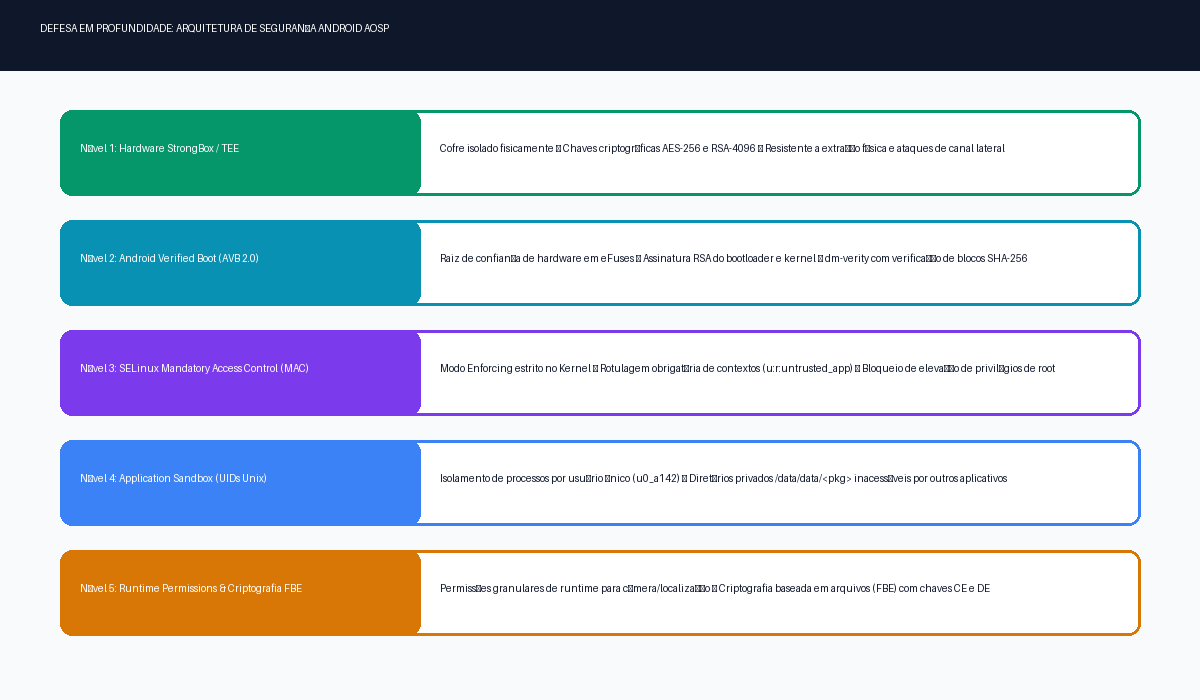
\includegraphics[width=0.95\textwidth]{imagens/fig_seguranca_fortress.png}
\caption{Defesa em Profundidade no AOSP: os 5 anéis concêntricos desde o Hardware StrongBox TEE e Verified Boot até o SELinux e a Sandbox por UID Unix.}
\label{fig:seguranca_fortress_img}
\end{figure}

\subsection{A Sandbox Baseada em UID Unix}
No Android, cada aplicativo instalado recebe um identificador de usuário Linux exclusivo (\texttt{UID}), por exemplo \texttt{u0\_a142} ($UID = 10142$). Sob a perspectiva do kernel, aplicativos diferentes são tratados como usuários distintos, sendo incapazes de acessar a memória ou os arquivos privados uns dos outros em \texttt{/data/data/<package>/}.

\subsection{Security-Enhanced Linux (SELinux): Mandatory Access Control}
A proteção por UID (\textit{Discretionary Access Control - DAC}) é insuficiente se um processo do sistema for comprometido por um exploit que obtenha permissões de superusuário (\textit{root}). O AOSP implementa o **SELinux** no modo **Enforcing** (\textit{Mandatory Access Control - MAC}):
\begin{itemize}
    \item Todo processo, arquivo, socket e nó de dispositivo possui um rótulo de segurança (\textit{Security Context}):
    \begin{equation}
        \texttt{user:role:type:sensitivity} \quad \text{ex.:} \quad \texttt{u:r:untrusted\_app:s0:c142,c256}
    \end{equation}
    \item Nenhuma ação é permitida a menos que exista uma regra explícita compilada na política do kernel:
    \begin{equation}
        \texttt{allow <origem> <destino>:<classe> \{ <permissões> \};}
    \end{equation}
\end{itemize}
Mesmo que um invasor obtenha root dentro do domínio \texttt{untrusted\_app}, o SELinux bloqueará qualquer tentativa de carregar módulos de kernel ou acessar nós de dispositivo não autorizados.

\subsection{Android Verified Boot (AVB 2.0) e Cadeia de Confiança}
O Verified Boot garante que nenhum código do sistema operacional tenha sido modificado:
\begin{enumerate}
    \item \textbf{Raiz de Confiança (Root of Trust):} Chave pública gravada fisicamente em fusíveis eletrônicos da ROM do processador (eFuses);
    \item \textbf{Cadeia Criptográfica:} A ROM de boot valida a assinatura do Bootloader, que valida a imagem de kernel (\texttt{boot.img}), que por sua vez valida a tabela de dispersão (\textit{hash tree}) do subsistema \texttt{dm-verity} das partições \texttt{system} e \texttt{vendor};
    \item \textbf{dm-verity:} Módulo de kernel que calcula o hash SHA-256 de cada bloco de disco de 4 KB sob demanda durante a leitura. Se um único byte for adulterado, o bloco é rejeitado e o kernel impede a inicialização.
\end{enumerate}

\subsection{Android Keystore \& Hardware StrongBox}
Para proteger chaves criptográficas mestras, o Android disponibiliza a camada do **Android Keystore**:
\begin{itemize}
    \item As chaves são geradas e operadas diretamente em um ambiente de execução confiável (\textit{Trusted Execution Environment - TEE / ARM TrustZone});
    \item O padrão mais elevado de proteção é o **StrongBox**: um chip de silício totalmente separado do SoC principal, com sua própria CPU, RAM e armazenamento resistente a violação física (\textit{tamper-resistant}).
\end{itemize}

\begin{lstlisting}[language=Java, caption={Geração de Chave AES-256 no Hardware StrongBox}]
val keyGenSpec = KeyGenParameterSpec.Builder(
    "SeldonMasterKey",
    KeyProperties.PURPOSE_ENCRYPT or KeyProperties.PURPOSE_DECRYPT
)
    .setBlockModes(KeyProperties.BLOCK_MODE_GCM)
    .setEncryptionPaddings(KeyProperties.ENCRYPTION_PADDING_NONE)
    .setUserAuthenticationRequired(true) // Exige biometria
    .setIsStrongBoxBacked(true)         // Aloca em chip Secure Element
    .build()

val keyGenerator = KeyGenerator.getInstance(
    KeyProperties.KEY_ALGORITHM_AES, "AndroidKeyStore"
)
keyGenerator.init(keyGenSpec)
keyGenerator.generateKey()
\end{lstlisting}

---

\section{Automação de Testes e Validações de Segurança (20h)}

\begin{pedagogico}{Objetivo Pedagógico da Disciplina}
Capacitar os residentes na construção de ferramentas automatizadas para auditoria de segurança móvel (DevSecOps), criação de scripts de validação contínua e tratamento formal de relatórios de vulnerabilidade com rastreabilidade de evidências.
\end{pedagogico}

\subsection{Integração DevSecOps Contínua}
A automação de testes de segurança busca eliminar vulnerabilidades ainda na fase de desenvolvimento (estratégia \textit{Shift-Left}):
\begin{itemize}
    \item Scripts em Python integrados à pipeline CI que decompilam o arquivo \texttt{AndroidManifest.xml} compilado via \texttt{aapt2} e verificam flags de risco:
    \begin{itemize}
        \item \texttt{android:debuggable="false"} obrigatório em builds de Release;
        \item \texttt{android:allowBackup="false"} para evitar extrações via \texttt{adb backup};
        \item \texttt{android:usesCleartextTraffic="false"} para impedir tráfego HTTP sem TLS 1.3.
    \end{itemize}
    \item Fuzzing automatizado de interfaces AIDL com geração estocástica de entradas malformadas para verificar resiliência a travamentos no AOSP.
\end{itemize}
